\addcontentsline{toc}{chapter}{Data Link e LAN}
\chapter*{\begin{center}\texttt{Datalink e LAN}\end{center}}
\hrulefill \\
\addcontentsline{toc}{section}{LAN}
\section*{\textcolor{RedViolet}{LAN}}
\noindent \underline{L}ocal \underline{A}rea \underline{N}etwork\\
\index{LAN}\index{data link}
\noindent LAN, Definizione del IEEE: Sistema di comunicazione che permette ad apparecchiature indipendenti di comunicare tra loro entro un'area delimitata, utilizzando un canale fisico ad elevata velocità e con basso tasso d'errore.\\

\begin{itemize}
    \item tipicamente, non sono trasmissioni di dati continue, ma a \openapex burst'', cioè a intervalli, a raffiche discontinue;
    \item tutte le macchine della LAN condividono lo stesso canale fisico di comunicazione;
    \item è una rete...
    \begin{itemize}
        \item economica;
        \item facile da modificare;
        \item di facile manutenzione;
        \item capace di sopportare grossi carichi di dati;
        \item duratura nel tempo (anni, se ben progettata e configurata).
    \end{itemize}
\end{itemize}
\noindent Aspetti meno piacevoli e delicati della LAN:
\begin{itemize}
    \item tutti gli host collegati devono essere identificati;
    \item bisogna stabilire delle regole per permettere agli host di comunicare tra di loro;
    \item flessibilità - compatibilità tra host di natura diversa (pensate ad un dispositivo mobile, un Desktop Computer, un sensore);
    \item modularità;
    \item espandibilità;
    \item gestibilità (vedere SNMP, protocollo Applicativo visto nel capitolo Application Layer);
\end{itemize}


\begin{wrapfigure}{r}{0.6\textwidth}
 \begin{center}
 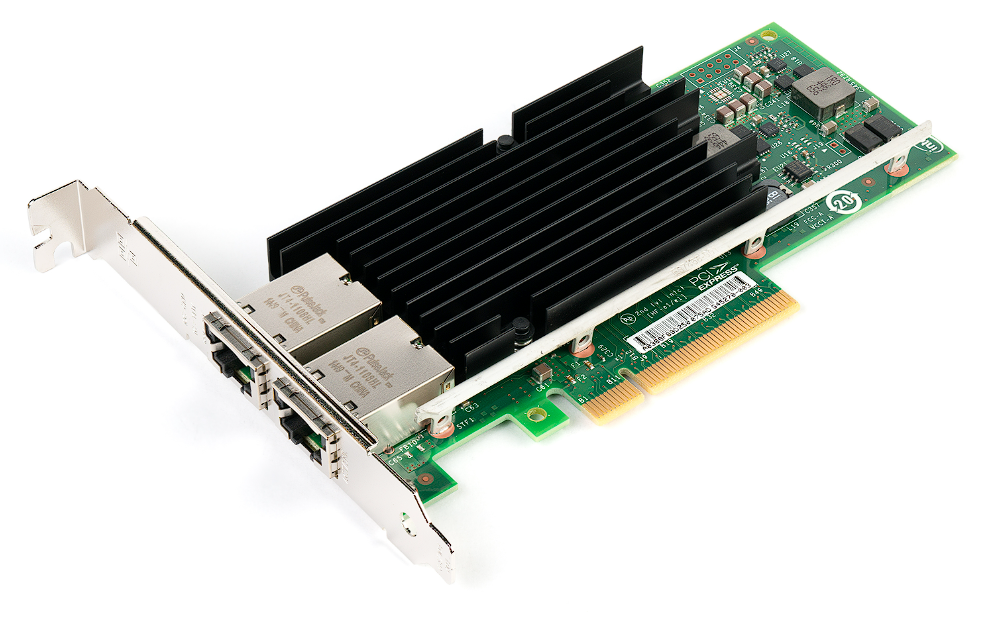
\includegraphics[width=1\linewidth]{Figures/05/nic.png}
  \end{center}
  \label{fig:nic}
  \caption{Una scheda di rete (NIC).}
\end{wrapfigure}


\noindent Cosa ci serve in una LAN?
\begin{itemize}
    \item beh, per iniziare, uno o più Host;
    \item software di rete (non necessariamente associato al sistema operativo);
    \item le NIC\index{NIC}(Network Interface Card, che possono essere cablate o wireless). Le schede di rete, fondamentalmente;
    \item delle API (Application Programming Interface), per interfacciarsi con il software;
    \item dei Network Hub, o Concentratori (e.g.: switch);
    \item cablaggio strutturato (cavi, antenne, etc.).
\end{itemize}

\noindent\textcolor{BlueViolet}{Le specifiche della LAN sono definite nello standard \hl{EIA/TIA 568} e \hl{ISO/EIC 11801}:\index{EIA/TIA 568} nello specifico, ISO/EIC 11801 definisce le specifiche del cablaggio standard. In genere, la sigla che volete ricordare è EIA/TIA 568.\\ \noindent \hl{IEEE 802.11} (anche questo va ricordato perché è uno standard importante) è il working group di IEEE che si occupa di gestire lo standard Wireless LAN; IEEE 802.3 invece si occupa dello standard Ethernet.\\}
\noindent LAN di solito è divisa in 2 macro categorie: Hardware (topologia, cavi, antenne tutto ciò che la rende funzionante sia per via cablata che wireless) e Software (tutti i protocolli e i software applicativi).

\addcontentsline{toc}{section}{Data Link}
\section*{\textcolor{Sepia}{Datalink}}
\index{data link}
\noindent Ovvero, il layer 2 dello stack TCP/IP.\\
\noindent A questo layer si riceve il messaggio dal layer di rete (quindi molto probabilmente si tratta di un messaggio IP), si struttura il messaggio al solito e lo si passa al layer sottostante (layer fisico, 1 nello stack). Con \openapex struttura il messaggio'' si intende questo: il messaggio IP viene suddiviso in frame delle dimensioni richieste dal layer sottostante, e gli viene aggiunta una FCS (Frame Check Sequence).\index{FCS}\\

\noindent Il layer Datalink si divide in:
\begin{itemize}
    \item LLC : Logical Link Control;\index{data link!LLC}
    \item MAC : Medium Access Control.\index{data link!MAC} Quest'ultimo è quello che si occupa di reperire informazioni su che tipo di mezzo fisico c'è al layer 1; funge anche da \openapex arbitro'' nella gestione del canale, perché nel momento in cui in rete si comunica con un canale unico diviso in broadcast sorge naturalmente il problema: come regolamentiamo l'accesso a questo canale? Occorre inventarsi un sistema che:
    \begin{itemize}
        \item Trovi gli indirizzi di tutti gli host connessi alla rete;
        \item Trovi, per ciascuno di questi indirizzi, il corrispondente indirizzo MAC (ora ci arriviamo, al MAC).
    \end{itemize}
\end{itemize}

\addcontentsline{toc}{subsection}{Frame Data Link}
\subsection*{La PDU del Datalink Layer: il Frame}
\index{frame!data link}
\noindent Un frame MAC contiene le seguenti informazioni:\begin{itemize}
    \item DSAP/SSAP: destination/source SAP (Service Access Point), sono i campi principali del frame, e sono indirizzi univoci a livello mondiale;
    \item payload: il corpo del messaggio da trasmettere;
    \item FCS: Frame Check Sequence, è un CRC\footnote{Controllo a Ridondanza Ciclica} su 32 bit, un sistema di controllo integrità tipo checksum.
\end{itemize}

\noindent Frame Ethernet: come di consueto, c'è una intestazione a cui segue il payload.\index{frame!ethernet}\\
\noindent Nell'header c'è quello che si chiama un preambolo: una sequenza di 7 byte tutti composti da $010101010101...$ (lungo $7\cdot8=56$ bit), seguito da un $8^o$ byte che, a differenza dei primi 7, è $01010111$ (quindi termina con `11'): il preambolo serve ad annunciare nel broadcast ``OK, questo è il segnale che adesso parlo io, quello che segue è il mio messaggio''. Seguono gli indirizzi del destinatario e del mittente, poi 2 byte che specificano la lunghezza del messaggio, poi il payload e il CRC.\\
\addcontentsline{toc}{subsection}{MAC}
\subsection*{Indirizzo MAC}
\index{MAC, indirizzo}
\noindent Lungo 48 bit (6 byte) formattati in 6 coppie \hl{esadecimali}:
\begin{verbatim}
    08:00:2b:3c:07:9a
\end{verbatim}

\begin{itemize}
    \item i primi 3 byte (nell'esempio, 08:00:2b) identificano il Vendor Code (detto anche OUI, Organization Unique Identifier). Standardizzati dal IEEE, sono codici associati ai produttori di schede di rete (e.g. Cisco);
    \item gli ultimi 3 byte (nell'esempio, 3c:07:9a) sono una numerazione progressiva decisa dai produttori. Questi identificano la scheda di rete $\approx$ \textit{\openapex questa è la scheda Wireless n° 101 prodotta da Cisco''}(è unica, come un numero di serie);
\end{itemize}

\noindent La scheda di rete\index{rete!scheda} può essere divisa in 2 componenti:
\begin{itemize}
    \item hardware (interfaccia di rete) (immagino qui mi riferissi alle cose come la porta Ethernet o l'ingresso per il cavo coassiale, le periferiche insomma);
    \item CPU + memoria - queste lavorano indipendentemente dal resto del PC, non elaborano dati da inviare al processore!
\end{itemize}

\noindent L'indirizzo fisico\index{indirizzo!fisico} deve essere \hl{unico nella LAN!} In Internet ci possono essere duplicati, ma in una rete locale non è ammesso. Normalmente, gli indirizzi fisici sono statici, tuttavia alle volte possono essere riassegnati.\\

\noindent L'indirizzo fisico può rappresentare:
\begin{itemize}
    \item UNICAST : un singolo host;
    \item MULTICAST : un gruppo di host;
    \item BROADCAST : tutte le stazioni (analogamente all'indirizzo IPv4, il MAC broadcast è della forma ff:ff:ff:ff:ff:ff, il più alto indirizzo possibile come 255.255.255.255). Nota: nel caso di un indirizzo broadcast, di norma il frame viene sempre analizzato (immagino per motivi di sicurezza);
\end{itemize}

\noindent Gli indirizzi di gruppo servono principalmente per fare neighbor discovery\index{neighbor discovery}(raccogliere info su chi altro è connesso alla rete). Vengono usati secondo due modalità di impiego:
\begin{itemize}
    \item solicitation: la stazione richiede un servizio e manda un messaggio multicast con l'indirizzo del servizio; le stazioni che offrono quel servizio, risponderanno ($\approx$ \textit{``mi serve questo, chi ce l'ha?''});
    \item discovery: le stazioni che offrono un servizio inviano, a cadenza regolare, un messaggio multicast per informare del servizio offerto ($\approx \textit{``ho questo, a chi serve?''})$
\end{itemize}

\noindent \textcolor{BlueViolet}{Comandi per neighbor discovery:}
\begin{verbatim}
        Linux terminal : ip neigh show
    Windows PowerShell : Get-NetNeighbor
\end{verbatim}

\noindent Esiste un protocollo di Network Discovery (chiamato appunto NDP), ma è configurato per IPv6.\\
\noindent Importante da ricordare: \hl{all'interno della LAN si comunica con indirizzi MAC, non IP!}\\
\noindent Protocolli \hl{ARP} e \hl{RARP}\index{ARP}\index{RARP}: stanno, rispettivamente, per Address Resolution Protocol e Reverse Address Resolution Protocol; ARP traduce l'indirizzo IP in indirizzo MAC, RARP passa da MAC a IP.

\addcontentsline{toc}{subsection}{Frammentazione dei Pacchetti IP}
\subsection*{IP e la Frammentazione dei Pacchetti}
\index{IP!frammentazione}
\noindent Nell'intestazione IP, ricordiamo, sono presenti alcuni campi come:
\begin{itemize}
    \item PROTOCOL (8 bit) : è l'informazione chiave che permette la lettura del payload - ovviamente, è quella che specifica che protocollo usare;
    \item HEADER CHECKSUM\index{header!checksum} : parity check, serve a controllare l'integrità del messaggio. Si prendono 16 bit dell'header e si fa il completamento a 1 della somma di tutti i 16 bit dell'header. Se tutto è corretto, il risultato è composto da tutti bit a $1$
    \item il 2° blocco di 32 bit dell'header IP è riservato alla frammentazione: identificativo, flags, fragment offset. La frammentazione è quel procedimento in cui un frame a livello datalink viene, appunto, frammentato in blocchi delle dimensioni richieste dal mezzo fisico di trasmissione sottostante (specificato nel MTU, Max Transmission Unit). Il riassemblaggio del frame viene effettuato solo una volta che questo ha raggiunto la destinazione, nonostante lungo il tragitto potrebbe passare per dei canali che ammettono delle MTU più grandi.
    Campi di frammentazione:
    \begin{itemize}
        \item primi 16 bit (di 32): identificativo;
        \item 3 bit seguenti: flags. Queste sono:
        \begin{enumerate}
            \item Bit riservato;
            \item Bit che, se posto a 1, significa \openapex non frammentabile'' (errore ICMP);
            \item Bit che, se posto a 0, significa \openapex questo frammento è l'ultimo (o l'unico) del datagramma);
        \end{enumerate}
        \item 13 bit finali : offset di frammentazione.
    \end{itemize}
\end{itemize}

\noindent Problematiche:
\begin{itemize}
    \item maggiore overhead (impiego di risorse non necessarie) di trasmissione;
    \item con la frammentazione è facile orchestrare attacchi DoS, mandando tantissimi pacchetti che costringono l'Host vittima ad impiegare molte risorse;
\end{itemize}
\noindent Questa funzionalità, propria di IPv4, in IPv6 non è presente.\\

\noindent\textcolor{Blue}{Note di Lab: esistono modi per calcolare la MTU più piccola possibile, dato un certo percorso di rete! Si può provare ad inserire in Wireshark il comando:}
\begin{verbatim}
    ping -f -l 193.205.92.2 // o qualche IP address, immagino
\end{verbatim}

\noindent\textcolor{Blue}{Fun fact: c'è qualche personaggio, appassionato di videogames e smacchinamenti di rete, che da qualche parte in qualche impostazione che non so, va a cambiare manualmente la dimensione di frammentazione dei PDU Ethernet da 1500 a 1473 (numero stranamente specifico, mah), questo perché sostengono che in questo modo si ottiene una velocità più elevata di navigazione, e questo aiuta a ridurre il ping in ms quando si gioca online. A detta del prof cambia poco e niente. (Beh, $1500-1473$ non è che sia chissà che miglioramento, in effetti)}\\

\noindent Dal momento che ogni router attraversato dal pacchetto ne modifica il Time-To-Live (che è un campo nel header IP), ogni volta va anche modificato il checksum (altrimenti se un campo cambia i conti non tornano più nella verifica. Che sbatta.)\\

\noindent\textcolor{Blue}{Note di Lab: per vedere su Wireshark la frammentazione, bisogna assicurarsi che nelle Preferenze il campo \openapex Reassemble...'' non sia selezionato. (Questo campo si trova sotto Protocols $>$ IPv4.)}\\

\addcontentsline{toc}{section}{Routing}
\section*{\textcolor{Cyan}{Routing - Instradamento}}
\index{routing}
\noindent Ovvero, tecniche ed algoritmi per fare in modo che i pacchetti arrivino a destinazione. ($\neq$ inoltro)\\N.B.: il router opera al layer 3 (IP).\\

\noindent Tabella di instradamento\index{instradamento!tabella}: è una specie di \openapex database'' memorizzato in un router o host; contiene le metriche dei costi, in termini di tempo, per poter valutare quale rete conviene attraversare da un host all'altro (come un GPS seleziona il percorso più breve, date location di partenza e destinazione).\\

\noindent Distinzione tra Routing e Forwarding:
\begin{itemize}
    \item Routing\index{routing}: insieme di regole per popolare queste tabelle;
    \item Forwarding\index{forwarding}: regole con le quali il pacchetto viene inviato a determinate porte di uscita del router (tipicamente questo viene fatto consultando le tabelle già popolate).
\end{itemize}

\noindent\textcolor{Blue}{Per stampare la tabella di routing, da terminale Windows PowerShell c'è il comando:}\begin{verbatim}
    > route print
\end{verbatim}
\index{routing!tabella}
\noindent Nelle tabelle di instradamento, per ogni sottorete, è elencato:
\begin{itemize}
    \item il relativo Network ID;
    \item l'indirizzo del router di inoltro;
\end{itemize}

\noindent Detta nel gergo dei database, i Record (i valori inseriti, i dati) nelle tabelle sono composti da: \begin{itemize}
    \item indirizzo della rete di destinazione;
    \item maschera di rete;
    \item l'interfaccia su cui inoltrare;
    \item l'indirizzo del next hop\index{next hop} (prossimo router da ragggiungere).
\end{itemize}

\noindent Ad ogni percorso è associata una metrica, ovvero un costo che può essere un'unità di tempo approssimato, oppure un numero di hop, dipende dal protocollo utilizzato.\\

\noindent Per il routing si usano 2 procedimenti:
\begin{itemize}
    \item Diretto: se l'host mittente è nella stessa rete del destinatario, inoltro direttamente al destinatario;
    \item Indiretto: gli host sono in due reti diverse, quindi dovrò inoltrare il messaggio ad uno o più router intermedi (quindi ci sarà almeno un next hop);
\end{itemize}

\noindent Domanda, però: come faccio a sapere se due host sono o meno nella stessa rete?\\
Tramite gli indirizzi IP degli host, risalgo agli indirizzi delle reti a cui i due rispettivamente appartengono: se i valori estratti corrispondono, allora si può procedere con instradamento diretto.\\

\noindent Per il routing\index{routing!diretto}\index{routing!indiretto} diretto si usa il MAC: coinvolge i layer 1 e 2 della stack;\\Per il routing indiretto si usa l'indirizzo IP del router, quindi i layer coinvolti della stack sono 1, 2 e anche 3 (IP).\\

\noindent La tabella di routing è \textit{sempre} presente in tutte le macchine che operano con IP, che siano Host o Router. Di solito la tabella contiene sempre almeno il next hop migliore, assieme ad altre cose. Il next hop è configurato in una sola direzione, tant'è che i percorsi di andata e ritorno sono asimmetrici di solito - la via del ritorno potrebbe prendere altre strade per arrivare al punto di partenza.\\

\noindent Tipi di rotte\index{rotte}:
\begin{itemize}
    \item statiche : configurabili dall'amministratore di rete;
    \item dinamiche : da reperire tramite protocollo di routing;
    \item dirette : legate alle interfacce del router.
\end{itemize}

\noindent Nota: si consideri la Figura \ref{fig:05interface}: quegli indicatori \openapex .1'' e \openapex.2'' stanno a specificare l'interfaccia di rete. Normalmente i router ne hanno più di una, quindi è buona abitudine specificare a quale di queste si fa riferimento ogni volta.

\begin{figure} [h]
    \centering
    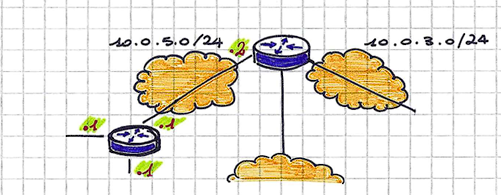
\includegraphics[width=0.8\linewidth]{Figures//05/interfacce.png}
    \caption{Dettaglio di un grafico di reti. Disegnato a mano da Yours Truly.}
    \label{fig:05interface}
\end{figure}

\newpage
\noindent La tabella di routing ha un aspetto del genere (stavolta fatta a mano perché è molto più carino spiegare ciascun campo così) (vedasi Fig. \ref{fig:routingtable}):

\begin{figure} [h]
    \centering
    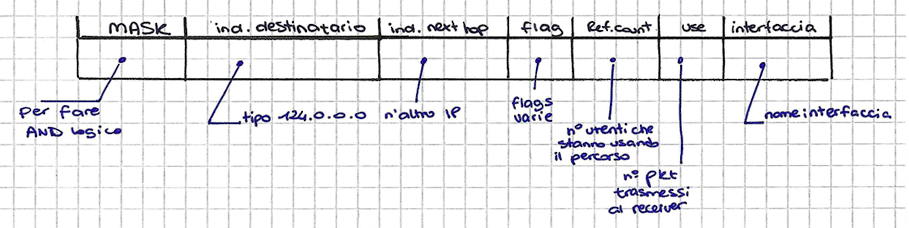
\includegraphics[width=1\linewidth]{Figures//05/routingtable.png}
    \caption{Dettaglio di un record di una tabella di routing. Di nuovo, cortesia di Yours Truly.}
    \label{fig:routingtable}
\end{figure}

\addcontentsline{toc}{subsection}{ICMP}
\subsection*{ICMP}
\index{ICMP}
\underline{I}nternet \underline{C}ontrol \underline{M}essage \underline{P}rotocol\\
incluso nello stack TCP/IP, è richiesto per qualsiasi implementazione standard di IP.\\

\noindent Fondamentalmente viene usato da IP per inviare messaggi di errore (per farlo, ICMP usa a sua volta IP. Meta! :D).\\


\begin{table}[h]
\centering
\begin{tabular}{ccc}
\multicolumn{3}{c}{Header ICMP (32 bit)}                                                                                    \\ \hline
\multicolumn{1}{|c|}{type (8 bit)} & \multicolumn{1}{c|}{code (8 bit)} & \multicolumn{1}{c|}{ICMP header checksum (16 bit)} \\ \hline
\end{tabular}
\end{table}

\noindent \openapex type'' specifica il formato, è un valore numerico associato a qualche informazione (e.g.: `0' = echo reply; `4' = source quench; `5' = redirect); \openapex code'' specifica il tipo di errore; il checksum è, di nuovo, il complemento a 1 di informazioni dell'header (IP, credo).\\

\noindent I messaggi sono di 2 tipi, fondamentalmente: segnalazione errori e richiesta informazioni.\\

\noindent Quando si usa il comando ``ping''\index{ping}, quello che succede è che viene creato un pacchetto ICMP di tipo ``8'', la risposta che arriva è un pacchetto ICMP di tipo ``1''.\\

\noindent Un altro tipo di messaggio era quello del ``timestamp'', serviva ad ottenere data e ora esatta segnata da certi host: ora questo servizio non si usa più perché tutti gli host usano il protocollo NTP (Network Time Protocol)\index{NTP}, che sincronizza gli orologi di tutti gli host al mondo con un orologio di riferimento.\\

\noindent Come funziona il \hl{Traceroute}\index{traceroute}:
\begin{itemize}
    \item il primo pacchetto è un messaggio ICMP con un TTL settato a 1: arriva al router immediatamente confinante, al che il TTL viene decrementato a 0 che innesca un messaggio ICMP di errore per TTL giunto a termine;
    \item il pacchetto seguente è di nuovo un messaggio ICMP con TTL settato a $1+1=2$: arriva al router immediatamente dopo, e si ripete la cosa del messaggio di errore;
    \item il processo viene ripetuto iterativamente con TTL incrementali così, in modo da ottenere info da tutti i router nel percorso. Fatto il traceroute :D
\end{itemize}

\noindent Protocolli di Routing AS (Autonomous Systems)\footnote{ASBR (Autonomous System Border Router)\index{ASBR}, router che tra le altre cose deve avere un'istanza sia dei router interni alla rete che di quelli esterni.}:
\begin{itemize}
    \item Protocolli inter-AS (esterni): BGP;
    \item Protocolli intra-AS (interni):
    \begin{itemize}
        \item \hl{distance vector}\index{distance vector}:
        \begin{itemize}
            \item RIP, RIP2\index{RIP}\index{RIP2};
            \item IGRP, EIGRP\index{IGRP}\index{EIGRP};
        \end{itemize}
        \item \hl{link state}\index{link state}:
        \begin{itemize}
            \item OSPF, OSPF2\index{OSPF}\index{OSPF2};
            \item IS-IS;
        \end{itemize}
    \end{itemize}
\end{itemize}

\noindent È importante che si sappia bene la differenza tra protocolli distance vector e protocolli link state, perché hanno degli scopi diversi!! I distance vector servono a trovare il percorso migliore tra router dato il numero di hop, i link state servono a scoprire com'è fatta la rete! Con i link state scopriamo tutte le rotte disponibili, con i distance vector scegliamo quella ottimale. Uno è puramente esplorativo, uno concerne l'ottimizzazione.\\

\addcontentsline{toc}{section}{Distance Vector}
\section*{Protocolli Distance Vector}
\index{distance vector!protocolli}
\noindent Vengono utilizzati per trovare il \hl{percorso migliore} nella rete, considerando come unità di misura il numero di hop tra un router e l'altro.\\

\noindent Fondamentalmente, ogni $x$ secondi, il router invia ai suoi vicini la propria routing table.\index{routing!tabella}\\
\addcontentsline{toc}{subsection}{Algoritmo RIP}
\subsection*{Algoritmo RIP}
\index{RIP!algoritmo}
\noindent \underline{R}outing \underline{I}nformation \underline{P}rotocol\\

\noindent\textcolor{Blue}{Differenza tra RIP e RIP 2: RIP era classful, RIP2 invece usa maschera (quindi è classless).}

\begin{enumerate}
    \item Consideriamo un router che al momento ha una tabella di routing così fatta:

\begin{table}[ht]
\centering
\begin{tabular}{ccc}
\multicolumn{3}{c}{Routing Table}                                                                                                   \\ \hline
\multicolumn{1}{|c|}{\textit{rete raggiungibile}} & \multicolumn{1}{c|}{n. Hop necessari} & \multicolumn{1}{c|}{router di origine:} \\ \hline
\multicolumn{1}{|c|}{Rete 1}                      & \multicolumn{1}{c|}{7}                & \multicolumn{1}{c|}{A}                  \\ \hline
\multicolumn{1}{|c|}{Rete 2}                      & \multicolumn{1}{c|}{2}                & \multicolumn{1}{c|}{C}                  \\ \hline
\multicolumn{1}{|c|}{Rete 6}                      & \multicolumn{1}{c|}{8}                & \multicolumn{1}{c|}{F}                  \\ \hline
\multicolumn{1}{|c|}{Rete 8}                      & \multicolumn{1}{c|}{4}                & \multicolumn{1}{c|}{E}                  \\ \hline
\multicolumn{1}{|c|}{Rete 9}                      & \multicolumn{1}{c|}{4}                & \multicolumn{1}{c|}{F}                  \\ \hline
\end{tabular}
\end{table}


    
    \item Il router riceve un messaggo da un certo Router C contenente la tabella di routing di C:

    \begin{table}[ht]
    \centering
    \begin{tabular}{cc}
    \multicolumn{2}{c}{Routing Table di C}                                                    \\ \hline
\multicolumn{1}{|c|}{\textit{rete raggiungibile}} & \multicolumn{1}{c|}{n. Hop necessari} \\ \hline
\multicolumn{1}{|c|}{Rete 2}                      & \multicolumn{1}{c|}{4}                \\ \hline
\multicolumn{1}{|c|}{Rete 3}                      & \multicolumn{1}{c|}{8}                \\ \hline
\multicolumn{1}{|c|}{Rete 6}                      & \multicolumn{1}{c|}{4}                \\ \hline
\multicolumn{1}{|c|}{Rete 8}                      & \multicolumn{1}{c|}{3}                \\ \hline
\multicolumn{1}{|c|}{Rete 9}                      & \multicolumn{1}{c|}{5}                \\ \hline
\end{tabular}
\end{table}
\item Il router prende queste informazioni, aumenta subito di 1 tutti gli hop dal Router C (l'hop che stiamo incrementando è il passo che serve per andare da questo router al router C);

\item La tabella ricevuta e incrementata viene ora comparata con quella che il router ha già: \begin{itemize}
    \item se la prima ha meno hop per raggiungere qualche rete, aggiorno quel campo con quello di C;
    \item se alcuni campi non erano presenti, vengono aggiunti (ad esempio, attraverso il router C ora possiamo raggiungere Rete 3);
    \item se il numero di Hop è lo stesso, è indifferente se aggiorniamo il campo della nostra tabella o no;
    \item se il numero di Hop è maggiore di quello che ho in tabella, non aggiorno la tabella con la nuova informazione;
\end{itemize}

\begin{table}[ht]
\centering
\begin{tabular}{ccc}
\multicolumn{3}{c}{Routing Table aggiornata}                                                                                        \\ \hline
\multicolumn{1}{|c|}{\textit{rete raggiungibile}} & \multicolumn{1}{c|}{n. Hop necessari} & \multicolumn{1}{c|}{router di origine:} \\ \hline
\multicolumn{1}{|c|}{Rete 1}                      & \multicolumn{1}{c|}{7}                & \multicolumn{1}{c|}{A}                  \\ \hline
\multicolumn{1}{|c|}{Rete 2}                      & \multicolumn{1}{c|}{5}                & \multicolumn{1}{c|}{C}                  \\ \hline
\multicolumn{1}{|c|}{Rete 3}                      & \multicolumn{1}{c|}{9 (nuovo)}                & \multicolumn{1}{c|}{C}                  \\ \hline
\multicolumn{1}{|c|}{Rete 6}                      & \multicolumn{1}{c|}{5 (sostituito 8F)}                & \multicolumn{1}{c|}{C}                  \\ \hline
\multicolumn{1}{|c|}{Rete 8}                      & \multicolumn{1}{c|}{4 (uguale)}                & \multicolumn{1}{c|}{C ( oppure E)}                  \\ \hline
\multicolumn{1}{|c|}{Rete 9}                      & \multicolumn{1}{c|}{4 (non aggiornato, $6>4$)}                & \multicolumn{1}{c|}{F}                  \\ \hline
\end{tabular}
\caption{Tabella di routing aggiornata. Nota: il valore di Rete 2 era 2 e proveniente da C, ma è stato aggiornato perché ora da C si arriva a Rete 2 con 5 hop.}
\end{table}
\item e questo è RIP.
\end{enumerate}

\addcontentsline{toc}{section}{Algoritmi di Instradamento}
\section*{Algoritmi di Instradamento}\index{instradamento!algoritmi}
\noindent O quella che il prof chiamò: Breve Carrellata di Algoritmi di Instradamento.\\

\noindent Il compito del livello di rete è di trasportare i pacchetti da un indirizzo di origine a un indirizzo di destinazione, ma non spetta a protocolli come IP occuparsi di come questo avviene fatto nella rete - di questo si occupano i Router! Di quale percorso far fare ai dati.\\

\noindent Riguardo il Forwarding diretto: all'interno dello stesso mezzo fisico possono esserci più reti a livello logico (pensate al subnetting con netmask): è compito del router occuparsi dell'instradamento anche lì tra quelle reti. In casi del genere è preferibile utilizzare una sola mega-rete che corrisponde alla topologia fisica. In casi quali? Immagino pensassi a casi in cui si fa spesso comunicazione interna, piuttosto che attraverso internet, non lo so sinceramente.\\

\noindent Protocollo Routabile (instradabile)\index{protocollo!instradabile}\index{protocollo!routabile}: protocollo che può essere utilizzato per applicare algoritmi di routing. Routing e Forwarding, utilizzati insieme, sono necessari per l'operatività di una rete. Informazione fondamentale a tale scopo è la tabella di routing.\\

\noindent Su tutte le macchine in cui è operativa la stack TCP/IP, siano essi End System o Router etc., è presente una tabella di routing ed esiste almeno un protocollo di routing.\\

\noindent Ciascun host è sempre collegato ad un default router, detto anche default gateway\index{default gateway}, detto anche first-hop router, detto anche router di primo rilancio, che comunica con la rete esterna.\\

\noindent Now onto our carrellata:
\begin{itemize}
    \item algoritmo di routing: trovare il miglior percorso da punto A a punto B ($\approx$ con il minor costo, data una certa misura tipo il nr Hop);
    \item Teoria dei Grafi (concetto visto nel corso di Algoritmi, tra le altre cose):
    \begin{itemize}
        \item Grafo\index{grafo}: un Grafo $\mathcal{G}=(\mathcal{N},\mathcal{E})$ è un insieme di $\mathcal{N}$ nodi ed $\mathcal{E}$ archi (dove E sta per Edges);
        \item Ad ogni arco che va dal nodo $x$ al nodo $y$ (arco $(x,y)$) è associato un costo $c(x,y)$;
        \item se il grafo non è orientato, allora vale sempre che gli archi sono uguali sia che vengono attraversati da x verso y che viceversa. $c(x,y) = c(y,x)$;
        \item $y$ è adiacente (o vicino) ad $x$ se esiste un arco che li collega: $(x,y)\in \mathcal{E}$;
        \item il costo complessivo di un percorso è la somma dei costi degli archi che lo compongono:
        \[c(x_1,x_n) = c(x_1,x_2)+c(x_2, x_3) +...+c(x_{n-1}, x_n)\]
    \end{itemize}
    \item 2 categorie di algoritmi di instradamento:
    \begin{itemize}
        \item statici: basati su tabelle manuali, percorsi che cambiano raramente;
        \item dinamici: la topologia della rete, i percorsi e i costi possono cambiare per cui bisogna adeguarsi spesso ai cambiamenti (questo viene fatto in base a un certo timer);
    \end{itemize}
    \item gli algoritmi si possono suddividere anche in queste due categorie:
    \begin{itemize}
    \item sensibili al carico: a seconda del carico della rete, cambierà la metrica;
    \item insensibili al carico: sono quelli utilizzati per la maggior parte (RIP, OSPF, BGP...)
    \end{itemize}
    \item ci sono altre due categorie che si possono usare come criterio:
    \begin{itemize}
        \item globali ($\approx$ link state): utilizzano tutti gli algoritmi a disposizione per conoscere l'intera mappa della rete. Per fare ciò, fanno quello che si dice \openapex flooding'' della rete;
        \item decentralizzati ($\approx$ distance vector): non c'è una conoscenza \textit{globale} della rete, solo dei nodi immediatemente vicini (più eventualmente il default gateway, ogni router ha conoscenza di se stesso!).
    \end{itemize}
\end{itemize}

\newpage
\addcontentsline{toc}{subsection}{Principio Distance Vector}
\subsection*{Principio Distance Vector}
\index{distance vector!principio}
\begin{figure} [ht]
    \centering
    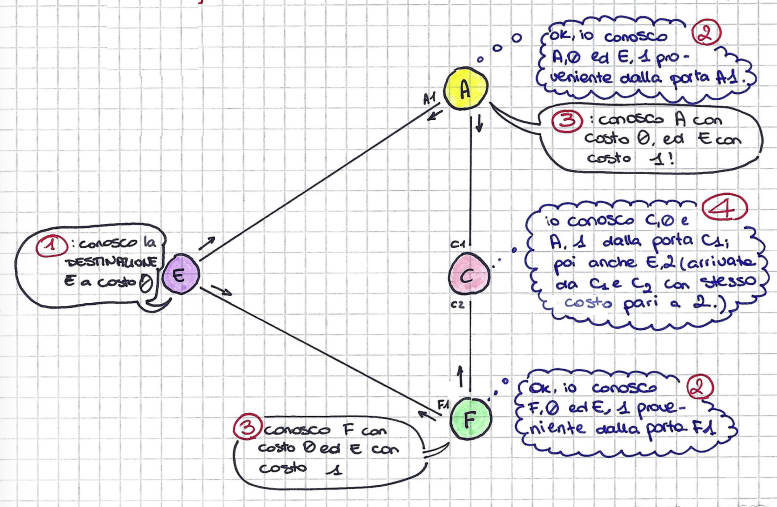
\includegraphics[width=0.8\linewidth]{Figures/05/distvec.png}
\end{figure}

\noindent Proprietà di:
\begin{itemize}
    \item distance vector:
    \begin{itemize}
        \item [+] semplici da implementare;
        \item [+] supportati da sistemi con scarse capacità di computazione e memoria;
        \item [-] problema del loop infinito (? anche se, stando alle mie note, questo è un problema che può essere risolto con il metodo ``split horizon''\footnote{vedere \href{https://www.techtarget.com/searchnetworking/definition/split-horizon}{qui :)}});
        \item [-] convergenza lenta (dipendente dal numero di nodi);
        \item [-] non possono usare molti hop (RIP ne ha massimo 15);
    \end{itemize}
    \item link state:
    \begin{itemize}
        \item [+] mappano la rete completamente;
        \item [+] non sono suscettibili a errori;
        \item [-] consumano moltissima banda (flooding);
        \item [-] non facilissimi da configurare;
        \item [-] richiedono capacità elevate in generale;
        \item [$\sim$] si usano in topologie dense di router.
    \end{itemize}
\end{itemize}

\noindent \textcolor{Blue}{La rete dell'università usa il protocollo link state OSPF.}\\

\noindent I pacchetti che il router invia per comunicare con gli altri le proprie informazioni si chiamano \openapex hello packet''.\\

\addcontentsline{toc}{section}{Algoritmi Link State}
\section*{Algoritmi Link State}
\index{link state!algoritmi}
\noindent Protocolli SSSP (Single Source Shortest Path):\begin{itemize}
    \item Algoritmo di Dijkstra;
    \item Algoritmo di Bellman-Ford;\footnote{differiscono essenzialmente per la metrica, se ho capito bene: il Bellman-Ford gestisce anche costi negativi, Dijkstra solo positivi.}
\end{itemize}
\addcontentsline{toc}{subsection}{Algoritmo di Dijkstra}
\subsection*{Alg. di Dijkstra}\index{Dijkstra!algoritmo}
\noindent L'algoritmo di Dijkstra si vede nel corso di Algoritmi, ragion per cui non lo approfondiremo troppo. Si consideri la rete in Fig. \ref{fig:dijkstra}, con i nodi che sono Router e gli archi che rappresentano il costo di ciascun collegamento:
\begin{figure} [ht]
    \centering
    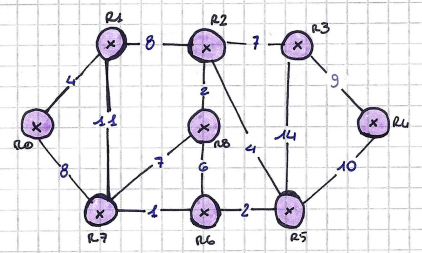
\includegraphics[width=0.75\linewidth]{Figures//05/dijkstra.png}
    \caption{Enter Caption}
    \label{fig:dijkstra}
\end{figure}

\begin{enumerate}
    \item Partiamo da $R_0$: i nodi che posso raggiungere e che scopro immediatamente sono $R_1$ con $c=4$ e $R_7$ con $c=8$;
    \item da $R_1$, $R_7$ posso scoprire $R_2$, $R_8$ e $R_6$;
    \item \textcolor{Red}{qual è il percorso meno costoso (che conosco ora) da $R_0$ a \{$R_2$, $R_8$, $R_6$\}}?
    \begin{enumerate}
        \item ($R_0\Rightarrow R_2$): $R_0\rightarrow R_1 \rightarrow R_2$ con costo $4+8=12$;
        \item ($R_0\Rightarrow R_8$): $R_0 \rightarrow R_1 \rightarrow R_2 \rightarrow R_8$ a costo $4+8+2=14$;
        \item ($R_0 \Rightarrow R_6$): $R_0\rightarrow R_7 \rightarrow R_6$ a costo $8+1=9$;
    \end{enumerate}
    \item da $R_2$, $R_8$, $R_6$ posso scoprire $R_3$ e $R_5$;
    \item \textcolor{Red}{qual è il percorso meno costoso (che conosco ora) da $R_0$ a \{$R_3, R_5$\}}?
    \begin{enumerate}
        \item ($R_0\Rightarrow R_3$): $R_0\rightarrow R_1 \rightarrow R_2 \rightarrow R_3$ a costo $4+8+7=19$;
        \item ($R_0 \Rightarrow R_5$): $R_0 \rightarrow R_2 \rightarrow R_6 \rightarrow R_5$ a costo $8+1+2=11$;
    \end{enumerate}
    \item infine, $R_0 \Rightarrow R_4$ si raggiunge via $R_0 \rightarrow R_7 \rightarrow R_6 \rightarrow R_5 \rightarrow R_4$ a costo $8+1+2+10=21$.
    \item Ci sono più percorsi possibili da $R_0$ ai vari router, ma questi che ho riportato sono i meno costosi!! Questo è ciò che ci interessa determinare. Tipo ($R_0\Rightarrow R_8$) passando per $R_0 \rightarrow R_1 \rightarrow R_7$, ma il costo sarebbe $4+11+7=22$;
\end{enumerate}

\begin{figure} [ht]
    \centering
    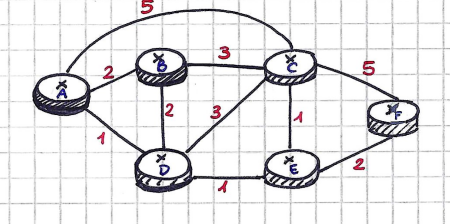
\includegraphics[width=0.75\linewidth]{Figures/05/dijkstra2.png}
    \caption{Altro esercizio da fare con Dijkstra.}
    \label{fig:dijk2}
\end{figure}

\noindent Al termine dell'esercizio proposto in Fig. \ref{fig:dijk2}, sperando che io non mi sia sbagliata, dovreste avere un risultato del genere:

\begin{table}[ht]
\centering
\begin{tabular}{|c|c|c|c|c|c|c|}
\hline
\textit{n. Hop da A} & Router attraversati & B   & C   & D   & E        & F        \\ \hline
0                    & A                   & 2,A & 5,A & 1,A & $\infty$ & $\infty$ \\
1                    & AD                  & 2,A & 4,D & -   & 2,D      & $\infty$ \\
2                    & ADE                 & 2,A & 3,E & -   & -        & 4,E      \\
3                    & ADEB                & -   & 3,E & -   & -        & 4,E      \\
4                    & ADEBC               & -   & -   & -   & -        & 4,E      \\
5                    & ADEBCF              & -   & -   & -   & -        & -        \\ \hline
\end{tabular}
\caption{Percorsi di minor costo da A alle varie direzioni.}
\end{table}

\begin{table}[ht]
\centering
\begin{tabular}{|c|c|c|}
\hline
\textit{destinazione} & next hop (passo 1) & costo \\ \hline
F                     & D                  & 4     \\
C                     & D                  & 3     \\
B                     & (B stesso)         & 2     \\
3                     & D                  & 2     \\
D                     & (D stesso)         & 1     \\ \hline
\end{tabular}
\caption{Tabella di Routing interna ad A.}
\end{table}


\addcontentsline{toc}{section}{Altro su Data Link e Ethernet}
\section*{Altre Cose su Data Link ed Ethernet}
\index{Ethernet}
\noindent In LAN, nel momento in cui un host trasmette nella rete, esso diventa proprietario di TUTTO il mezzo trasmissivo! (nel senso che, fintanto che è lui a parlare, è lui a monopolizzare il canale). Questo era un problema di sicurezza ``non indifferente'' agli albori della tecnologia LAN, il fatto che tutti i messaggi fossero broadcast, a cui si è in qualche modo ovviato con CSMA-CD, che vedremo in un attimo.\\
\noindent Con il termine Ethernet ci si riferisce sia alla tecnologia per connettere dispositivi in LAN (cablaggio e porte, immagino), sia ad una componente logica, algoritmica se vogliamo, utilizzata per gestire le trasmissioni di dati su questa rete. In altre parole, sentiamo parlare sia di ``Cavo Ethernet'' (tecnologia fisica) che di ``Frame Ethernet'' (tecnologia logica, come un Pacchetto IP).\\

\noindent Memo degli standard e di chi li ha pubblicati (cercate di ricordarveli questi, sono importanti):\index{standard!IEEE 802}
\begin{itemize}
    \item IEEE 802 : definisce diversi standard LAN, tra cui quelli più rilevanti sono:
    \begin{itemize}
        \item 802.3 : Ethernet;
        \item 802.11 : WLAN (Wireless LAN) \textit{\& Mesh (Wi-Fi certification)} (qualsiasi cosa significhi ciò);
        \item gli altri punti di IEEE 802 sono stati dismessi, come ad esempio 802.5 che definiva la topologia Token Ring (ampiamente in disuso oggi).
    \end{itemize}
    \item EIA/TIA 568\index{standard!EIA/TIA 568} : definisce gli standard per il cablaggio strutturato (e.g. come vanno disposti i cavi colorati all'interno della spina RJ-45 ad un estremo e all'altro del cavo Ethernet\index{Ethernet!cavo}, se si vogliono creare cavi Straight-Through o Crossover, questo lo vedremo nel prossimo capitolo);
\end{itemize}

\noindent Di nuovo, giusto per ripetermi: a livello Data Link, la PDU prende il nome di Trama o Frame (quindi per esempio si parla di ``Frame'' Ethernet).\\
\index{Ethernet!frame}
\noindent La struttura del Frame Data Link dipende dalla tecnologia fisica sottostante, pertanto non c'è uno standard unico ben preciso sulla struttura di un Frame. In linea generica, però, le sue dimensioni sono comprese tra $64\div 1518$ Bytes, e tra le informazioni trasmesse ci sono:
\begin{itemize}
    \item un trailer all'inizio, che contiene indirizzi di destinatario e mittente;
    \item il payload;
    \item una forma di rilevazione errori come CRC\index{CRC}, controllo a ridondanza ciclica, o controllo di parità i somme di controllo;
\end{itemize}

\noindent I collegamenti possono essere fondamentalmente di 2 tipi:
\begin{itemize}
    \item Broadcast : più stazioni connesse con lo stesso mezzo trasmissivo;
    \item Point to Point : cablato o wireless, collega una stazione ad una stazione e basta. (in casi come questo viene utilizzato il cavo Cross-Over, e più in generale ogniqualvolta si intende collegare tra loro due dispositivi dello stesso tipo, Router a Router, Host a Host...)
\end{itemize}

\noindent In caso di reti ad accesso multiplo (LAN, reti via satellite...), sono richiesti protocollo ad accesso multiplo per dirigere il traffico senza causare collisioni\index{collisioni}. Questi possono operare per:
\begin{itemize}
    \item suddivisione del canale in TDM/FDM (come dicevamo nell'introduzione, dividere la banda comune in slot di tempo o di frequenza) ($\approx$ Channel Partitioning Protocols);
    \item accesso casuale (RAP, Random Access Protocols), come lo Slotted ALOHA;
    \item a rotazione (taking-turn protocols), in cui gli host parlano a turno secondo diversi criteri come Polling o Token-Passing. 
\end{itemize}

\noindent Tecniche di allocazione del canale trasmissivo:
\begin{itemize}
    \item statica: il mezzo viene partizionato tipo TDM/FDM;
    \item dinamica: tutte le frequenze del mezzo trasmissivo vengono assegnate di volta in volta ai vari host (nel caso dei protocolli turn-based, naturalmente, occorre definire un algoritmo che gestisca questa assegnazione dinamica).
\end{itemize}

\newpage
\noindent Sketch originale\index{Ethernet!tecnologia} (riprodotto da me, ofc) della tecnologia Ethernet, ideata nel 1976 da Metcalfe:\\
\begin{wrapfigure}{l}{0.6\textwidth}
 \begin{center}
 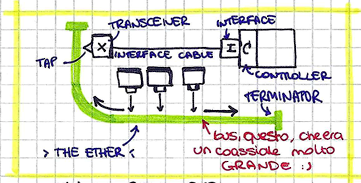
\includegraphics[width=1\linewidth]{Figures/05/ethernet1976.png}
  \end{center}
  \label{fig:eth1976}
\end{wrapfigure}

\begin{itemize}
    \item c'è un solo bus condiviso (in origine, un cavo coassiale);
    \item  è non-deterministico - non c'è nessuna regola che stabilisce quando parla chi (quindi ci si chiede: quando e dove si trasmette sul bus?)
    \item ad oggi, Ethernet è la tecnologia cablata più diffusa, si è passati da una topologia a Bus come quella nello sketch ad una topologia a stella (switched Ethernet\footnote{vedremo poi che si è passati all'utilizzo del cosiddetto Ethernet Hub, che comunque contiente una forma di Bus al suo interno})
\end{itemize}

\noindent Topologia a Bus:\index{topologia!a bus}
\begin{itemize}
    \item 
interruzione del bus in qualsiasi punto $\rightarrow$ interruzione di tutta la rete;
\item aggiungere un end system alla rete comporta un grosso intervento, con interruzione del servizio nell'intero sistema;
\item un frame immesso nel bus si propaga ogni volta in entrambe le direzioni del bus.
\end{itemize}

\noindent Aloha\index{Aloha}: protocollo per topologie a Bus (indovinate in che paese è stato ideato). Consente trasmissione in modo casuale, quindi spesso i frame mandati in rete allo stesso momento andavano in collisione! Collisioni che potevano essere parziali o totali, a seconda della \% di timeslot sovrapposti tra i messaggi in conflitto. È un protocollo facile da realizzare, ma naturalmente presenta dei problemi di efficienza.

\addcontentsline{toc}{subsection}{CSMA: Gestione Collisioni}
\subsection*{CSMA}\index{collisioni!CSMA}
\noindent \underline{C}arrier \underline{S}ense \underline{M}ultiple \underline{A}ccess, dove Carrier Sense è un modo per dire, più o meno: ``prima di parlare, ascolta.'' (e mentre trasmetti, continua ad ascoltare)

\begin{itemize}
    \item CSMA-CA: Collision Avoidance;
    \item CSMA-CD: Collision Detection.
\end{itemize}

\noindent Ma! Neppure l'utilizzo dei protocolli CSMA-CA/CD scongiura del tutto le collisioni.\\
\noindent Supponete che per caso inizino a parlare 2 End Systems in contemporanea: collidono una volta, si fermano entrambi e lasciano parlare l'altro, tipo la scena cliché in cui due persone iniziano a dire entrambe ``no scusa, vai prima tu'' e così facendo parlano assieme di nuovo e avanti così più e più volte.\\
\noindent Come si scongiura questa situazione di stallo infinito deadlock? Si tenta di dire, al momento della collisione, agli host di aspettare un tempo $T$ generato randomicamente: questa istruzione di aspettare viene data attraverso un segnale speciale (``jamming'') che ha una certa frequenza;\\
\noindent Se, disgraziatamente, i tempi randomici scelti dalle parti coinvolte sono di nuovo uguali e c'è di nuovo interferenza, si raddoppia il range di tempi T di attesa da scegliere a caso! Nel senso: se alla prima collisione avrei aspettato un tempo nell'insieme I$\mathcal{T}=\{0,1\}$, la seconda volta sceglierò tra $\mathcal{T}' = \{0,1,2,3\}$: più elementi ci sono nell'insieme $\mathcal{T}$, minore è la probabilità che 2 End System peschino lo stesso $t$. Questo meccanismo si chiama ``Exponential Backoff''.\index{collisioni!exponential backoff}\\

\noindent Andiamo avanti. Dominio:\index{dominio}
\begin{itemize}
    \item di Broadcast: parti di rete in cui il messaggio broadcast riesce a raggiungere tutti gli host: nel caso di una LAN, il dominio di BC e limitato dal Router (Gateway).
    \item di Collisione: parti della rete dove c'è la possibilità che si verifichino collisioni.
\end{itemize}

\noindent Tempo per rilevare una collisione:
\[a = \dfrac{\text{lunghezza\_collegamento}}{\text{lunghezza\_pkt}}\]